\documentclass[12pt, a4paper, twoside]{article}
\usepackage{labreport}
\usepackage{pdfpages}

\setlabreportopts[authors={Nandor Kovacs \& Céline Schuster},
    title={Mathematisches Pendel},
    subtitle={Untersuchung der Eigenschaften eines Mathematischen Pendels},
    date={\today},
    labdate={4. März 2022}
]

\begin{document}
\maketitlepage

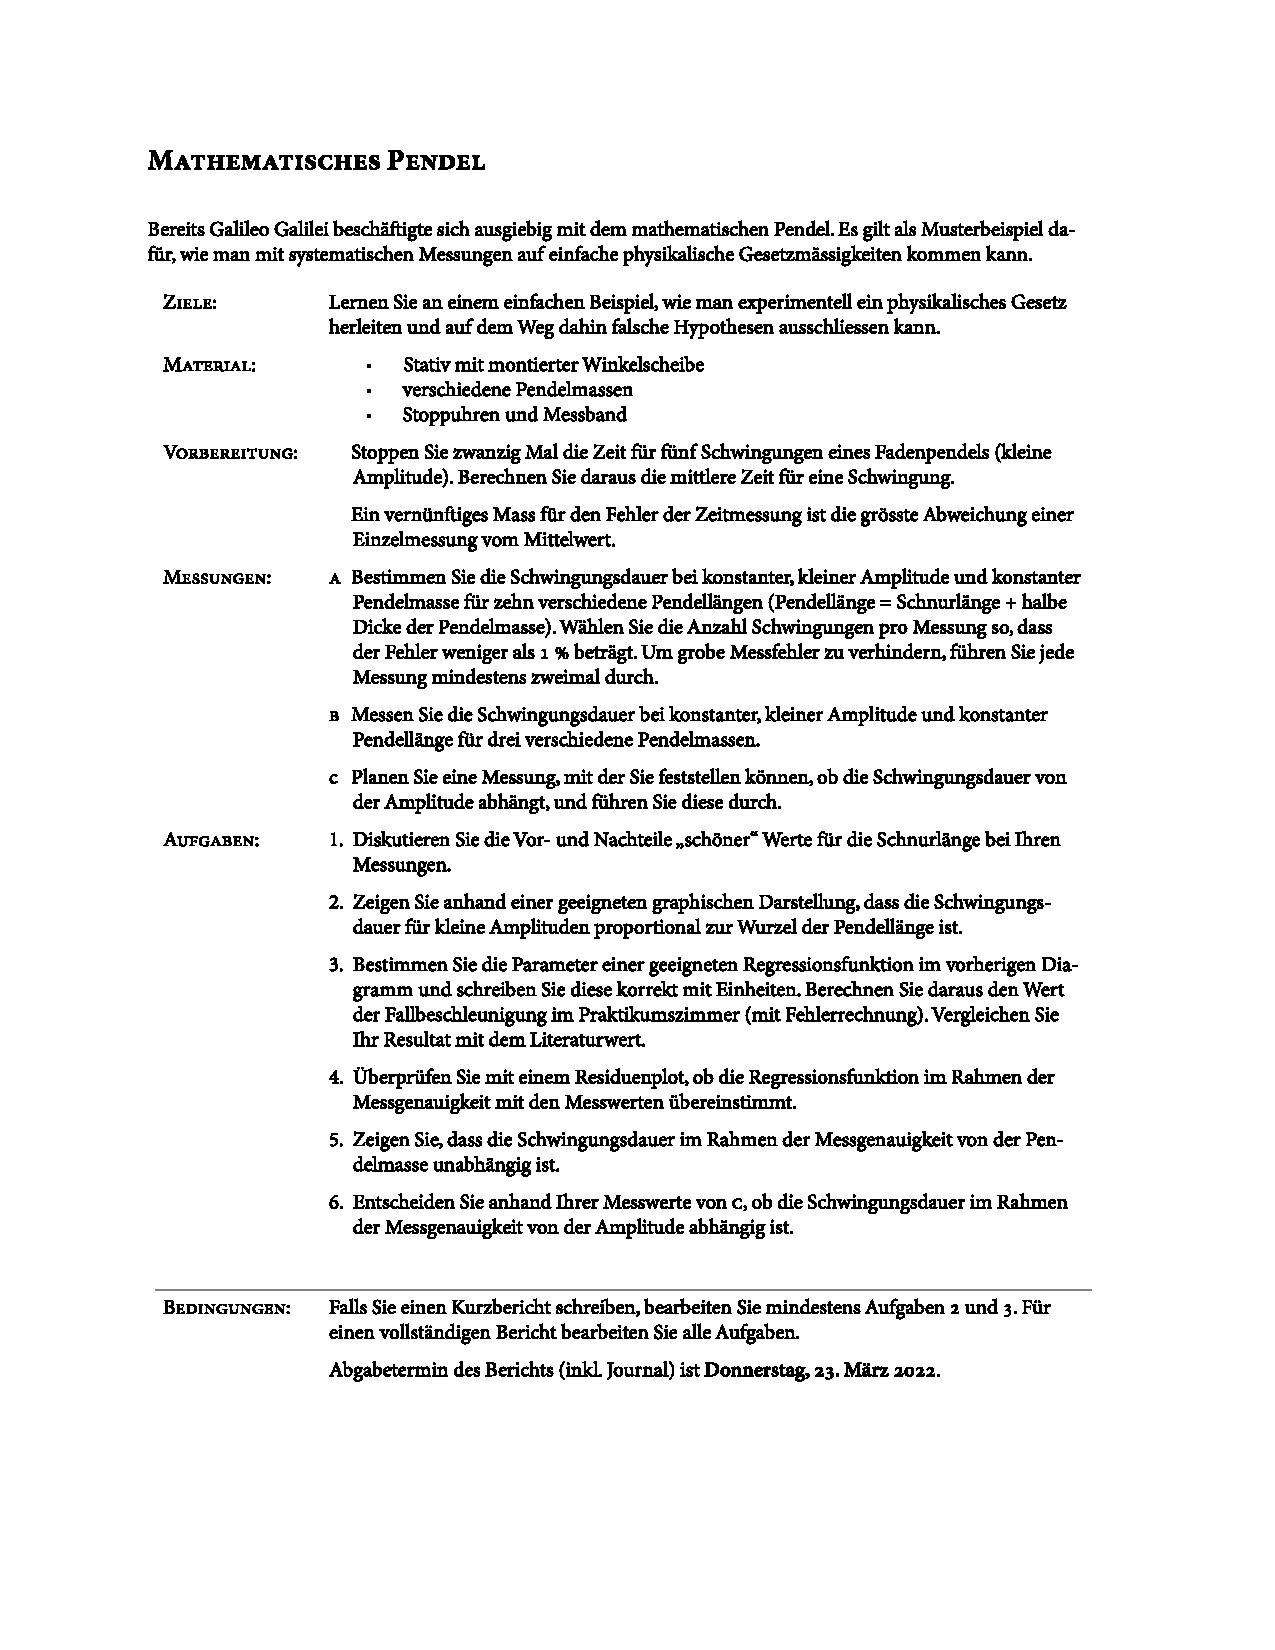
\includepdf[pages={1}]{aufgabenstellung.pdf}

\section{Einleitung}
Wir alle kennen Pendeluhren.
Pendeluhren benutzen statt Quartz stückchen, oder Signale von einer Radiouhr eine Pendel um die Zeit zu verfolgen.
Das muss heissen, das die Periodenlängen von Pendeln berechenbar sind.
Falls die Periode von dem Ausschlagwinkel abhängt, würde das aber recht kompliziert sein zum berechnen, also vermuten wir dass das nicht der Fall ist.

\section{Theorie}
Eine Pendel hat folgende Parameter:
\begin{list}{-}{}
  \item \emph{l} = die Länge der Pendel
  \item \emph{g} = das Gewicht des Pendelgewichts. Dies ist gleich zur länge der Schnur plus die halbe Dicke des Gewichts.
  \item \emph{$\alpha$} = die auslenkung beim starten der Pendel in winkelgrad
\end{list}

Die Formel für die länge einer Periode in Sekunden lautet
$$T=2\pi\cdot\sqrt{\frac{l}{g}}$$
\cite{FoTa}

\section{Experiment}
\begin{figure} [ht]
  \centering
  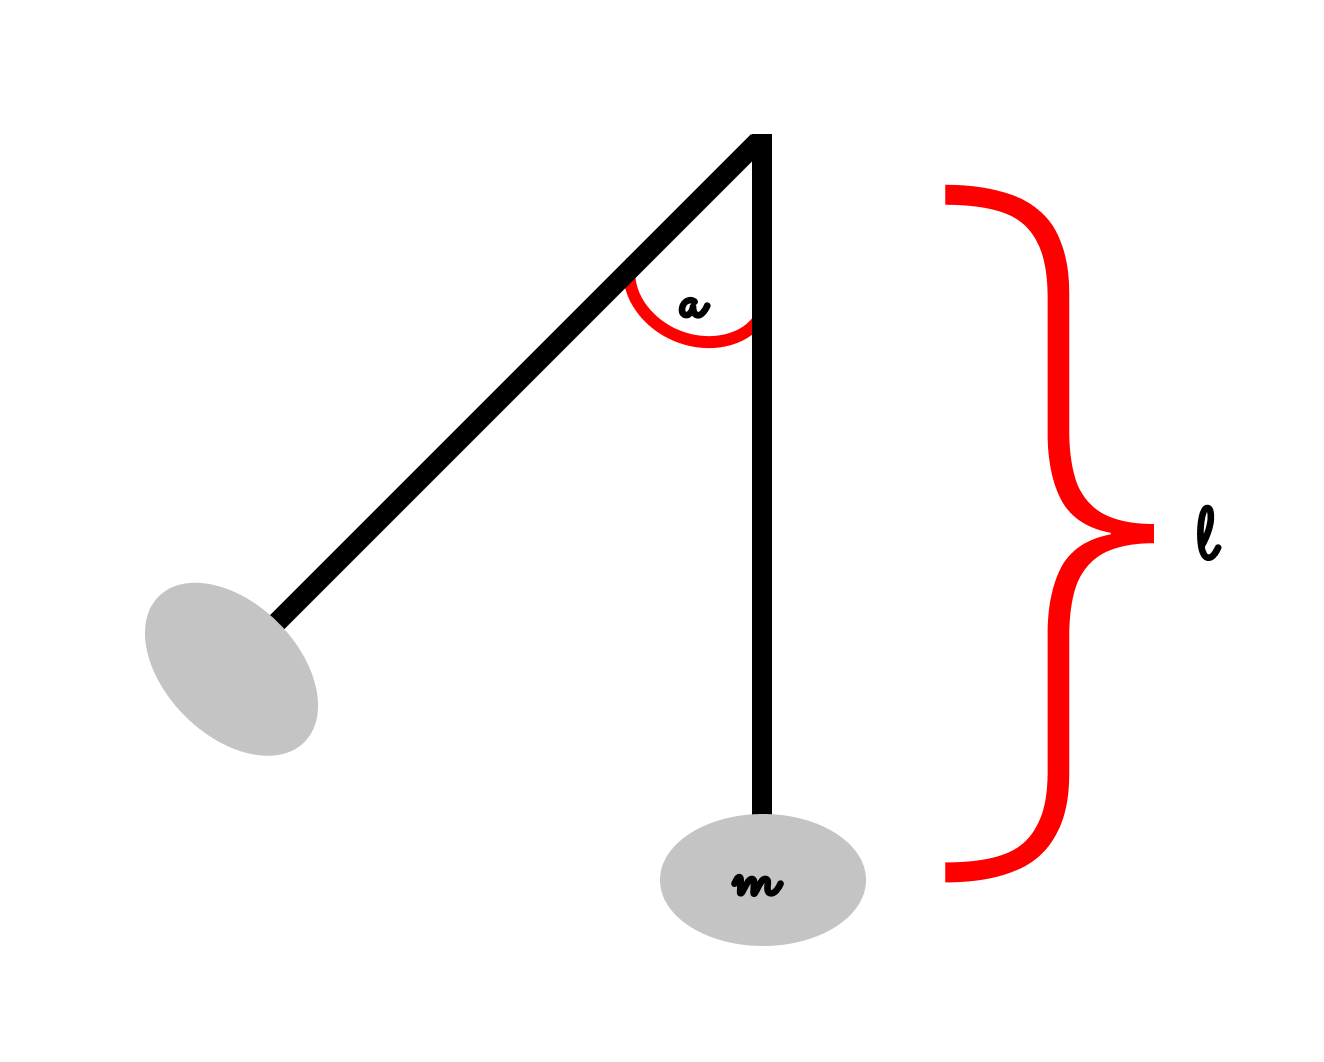
\includegraphics[width=0.5\textwidth]{Experimentaufbau.png}
  \caption{Skizze Experimentaufbau}
  \label{fig:experimentaufbau}
\end{figure}

Unser Experiment ist einfach aufgebaut.
Es wird ein Gewicht an einem Faden Aufgehängt.
Sie wird ausgelenkt, losgelassen, und die Zeit der Perioden werden gemessen wenn das Gewicht die Mitte kreuzt.
Wir lassen ausserdem 5mal das Gewicht pendeln bevor wir es messen, damit ungenauigkeiten ausgependelt werden.

Die länge $l$ messen wir mit einem Massband auf 0.5cm genau und $\alpha$ messen wir mit einer Winklerscheibe auf 2\textdegree genau.
Die Zeit messen wir mit einer Stoppuhr.

Um die genauigkeit von den Zeitmessungen zu bestimmen, messen wir 20mal mit dem gleichen $\alpha$, $m$, und $l$.
Wir berechnen die maximale Abweichung mit diesen Daten.

\datatable{2}{Messungen zur Vorbereitung}{Nr. & Periodenlänge $T$ in s}{Messung_a.csv}


\begin{align*}
  \overline{T} & = \frac{1}{n} \sum_{i=1}^{n} T_{i}=\frac{1}{n}\left(T_{1}+\cdots+T_{n}\right) \\
               & =\frac{164.01s}{20}                                                           \\
               & =8.2005s                                                                      \\
  \\
  \Delta T     & = max(T_{max} - \overline{T}, \overline{T} - T_{min})                         \\
               & = max(8.27s - 8.2005s, 8.2005s - 8.14)                                        \\
               & = 0.0695s                                                                     \\
               & = 0.07s
\end{align*}

\vfill\pagebreak

\section{Messungen}
\datatable{2}{$m$ ist konstant, $\alpha$ ist konstant und klein, $l$ ist variabel}{Pendellänge $l$ in cm & Periodenlänge $T$ in s}{laenge.csv}
\datatable{2}{$l$ ist konstant, $\alpha$ ist konstant und klein, $m$ ist variabel}{Gewichtsmasse $m$ in g & Periodenlänge $T$ in s}{masse.csv}
\datatable{2}{$l$ ist konstant, $m$ ist konstant, $\alpha$ ist variabel}{Amplitude $\alpha$ in Winkelgrad & Periodenlänge $T$ in s}{winkelgrad.csv}

\section{Aufgaben}
\subsection{Vor und Nachteile schöner Werte für $l$}
Schöne längen für $l$ sind einfacher zu messen, was ein deutlicher vorteil ist.
Das Problem ist, das wenn $l$ einen schönen Wert hat, dann wird $T$ relativ sicher keinen schönen Wert haben.

\subsection{Proportionalität von $T$ zu $l$}

\pgfkeys{
  /datadiagram/.is family, /datadiagram,
  x label/.store in=\xlabel,
  x data/.store in=\xdata,
  x error/.store in=\xerror,
  y label/.store in=\ylabel,
  y data/.store in=\ydata,
  y error/.store in=\yerror,
}

\pgfkeys{/datadiagram, x data=l,
  x label=Pendellänge $l$ in cm,
  x error=0.1,
  y label=Periodenlänge $T$ in s,
  y data=T,
  y error=0.0
}
\begin{center}
  \begin{tikzpicture}
    \begin{axis}[
        axis lines = left,
        enlargelimits=0.2,
        ylabel={\ylabel},
        xlabel={\xlabel},
        cycle list name=black white
      ]
      \addplot+[color=red, domain=0:125, samples=100, mark=none]{sqrt(x)};
      \addlegendentry{sqrt(x)}
      \addplot+[only marks] table[x=\xdata, y=\ydata, col sep=comma] {laenge.csv};
      \addlegendentry{unsere messungen}
    \end{axis}
  \end{tikzpicture}
\end{center}

Diese Grafik illustriert gut das $T$ proportional zur Wurzel von $l$ ist. 

\subsection{Abhängigkeit Schwingsungsdauer und Amplitude}
\datatable{2}{Messungen zu Aufgabe c}{Amplitude $\alpha$ in \textdegree & Schwingungsdauer $T$ in s}{Messung_c.csv}

\datadiagram[x label=Amplitude $\alpha$ in \textdegree,
  x data=alpha,
  x error=2,
  y label=Schwingungsdauer $T$ in s,
  y data=T,
  y error=0.2
]{Messung_c.csv}

Auch hier sind die Differenzen kleiner als der Messfehler, daher können wir auch annehmen, dass die Schwingungsdauer von der Maplitude unabhängig ist.

\subsection{Schwingungsdauer als Funktion der Pendellänge}
\datatable{2}{Messungen zu Aufgabe d}{Pendellänge $l$ in cm & Schwingungsdauer $T$ in s}{Messung_d.csv}
\datadiagram[x label=Pendellänge $l$ in cm,
  x data=l,
  x error=0.1,
  y label=Schwingungsdauer $T$ in s,
  y data=T,
  y error=0.2
]{Messung_d.csv}

\section{Fazit}
\section{Reflektion}
\section{Referenzen}
\printbibliography[heading=none]
\section{Anhang}
Veruschsanleitung und Originalprotokoll vom \labdate

\end{document}